\documentclass[dvipsnames]{fairmeta}

\title{The Llama 3 Herd of Models}

\author[1]{Llama Team, AI @ Meta}
\affiliation[1]{A detailed contributor list can be found in the appendix of this paper.}

\abstract{
Modern artificial intelligence (AI) systems are powered by foundation models.
This paper presents a new set of foundation models, called Llama 3.
It is a herd of language models that natively support multilinguality, coding, reasoning, and tool usage.
Our largest model is a dense Transformer with 405B parameters and a context window of up to 128K tokens.
This paper presents an extensive empirical evaluation of Llama 3.
We find that Llama 3 delivers comparable quality to leading language models such as GPT-4 on a plethora of tasks.
We publicly release Llama 3, including pre-trained and post-trained versions of the 405B parameter language model and our Llama Guard 3 model for input and output safety.
The paper also presents the results of experiments in which we integrate image, video, and speech capabilities into Llama 3 via a compositional approach.
We observe this approach performs competitively with the state-of-the-art on image, video, and speech recognition tasks.
The resulting models are not yet being broadly released as they are still under development.
}

\date{July 23, 2024}

\metadata[Website]{\url{https://llama.meta.com/}}

\usepackage{makecell}
\usepackage{siunitx}
\usepackage{framed}
\usepackage{pifont}
\usepackage{graphicx,subcaption}
\usepackage{pifont}
\usepackage{xspace}
\usepackage{nicematrix}
\usepackage{nicefrac}
\usepackage{wrapfig}
\newcommand{\rulesep}{\unskip\ \vrule\ }
\newcommand{\cmark}{\textcolor{ForestGreen}{\ding{51}}}
\newcommand{\xmark}{\textcolor{red}{\ding{55}}}

\begin{document}

\maketitle

\providecommand{\llama}{Llama\xspace}
\providecommand{\llamatwo}{Llama~2\xspace}
\providecommand{\llamathree}{Llama~3\xspace}
\providecommand{\TODO}[1]{{\color{red}[\textbf{TODO}: #1]}}
\providecommand{\mlc}{Multilingual\xspace}
\providecommand{\gpt}{GPT-4\xspace}
\providecommand{\gptp}{GPT-4\xspace}
\providecommand{\gpto}{GPT-4o\xspace}
\providecommand{\gptfourturbo}{GPT-4 Turbo\xspace}
\providecommand{\sonnet}{Claude 3.5 Sonnet\xspace}
\providecommand{\nemotron}{Nemotron 4 340B\xspace}
\providecommand{\mixtralbig}{Mixtral 8$\times$22B\xspace}
\providecommand{\gptthreedotfivet}{GPT-3.5 Turbo\xspace}
\providecommand{\gemmatwo}{Gemma 2 9B\xspace}
\providecommand{\mistralsmall}{Mistral 7B\xspace}
\providecommand*{\acc}[1]{\num[round-mode=places,round-precision=2]{#1}}


\section{Introduction}
\label{sec:introduction}

\begin{wrapfigure}{r}{0.5\textwidth}
\vspace{-6mm}
\begin{center}
    \includegraphics[width=0.5\textwidth]{images/cover.pdf}
  \end{center}
  \vspace{-4mm}
  \caption{\textbf{Overview of \implname.} In training, we tune the singular values of the weight matrices to generate a set of ``expert'' vectors specializing in different tasks. In inference, a two-pass process is adopted where the first applies the expert and the second generates the answer.}
  \label{fig:cover}
  \vspace{-4mm}
\end{wrapfigure}

Self-adaptive large language models (LLMs) would represent a significant advancement in artificial intelligence, enabling real-time adaptation to various tasks and contexts.
While compositionality and scalability are crucial for effective adaptation, current LLM training methodologies fall short of achieving both these properties simultaneously.
Our research aims to present a solution to address these gaps.

In principle, the first step toward achieving self-adaptive LLMs can be realized through the development of specialized expert modules, each fine-tuned~\citep{kaplan2020scaling} via techniques such as low-rank adaptation (LoRA)~\citep{hu2021lora}. 
However, several challenges need to be addressed to make this approach both scalable and compositional: (1) multiple expert modules significantly increase the number of parameters; (2) expert modules are often prone to overfitting; and (3) flexible composition of these experts is still an open problem.

To overcome these limitations, we first propose \svdacro, a novel parameter-efficient fine-tuning (PEFT) method to obtain effective building blocks for self-adaptation.
\svdacro works by extracting and selectively tuning only the singular values within the model's weight matrices.
By focusing on this essential and principled parameterization, our approach mitigates the risk of overfitting, drastically reduces computational demands, and allows for inherent compositionality.

We then introduce our full \implname framework, which entails a two-pass inference mechanism to produce dynamically adapted weights targeted for the test-time conditions (Figure~\ref{fig:cover}).
We design three different adaptation strategies that can be used within \implname, which we show provide monotonic performance benefits with increasing access to the test-time conditions.
We evaluate \svdacro and the full \implname framework through extensive experiments across a diverse range of LLMs and tasks.
\svdacro outperforms traditional efficient fine-tuning methods like LoRA on domain-specific datasets with far fewer parameters. 
\implname further improves performance, even for out-of-distribution tasks like visual QA. 
Our analysis even shows that \implname allows the reuse of \svdacro experts across different LLMs. In summary, our key technical contributions are: 
\vspace{-2mm}
\begin{itemize}
\item The development of \implname as a pivotal self-adaptation framework for LLMs, providing a blueprint to adapt the behavior of LLMs from a growing set of pre-trained skills.
\item The introduction of \svdacro, a novel PEFT method trainable with RL on small datasets, producing compact expert vectors with inherent compositionality.
\item The implementation of three adaptation strategies, effectively dispatching \svdacro-trained experts with properties designed to cope with different deployment scenarios.
\end{itemize}

\vspace{-2mm}
\begin{figure*}[t]
    \centering
    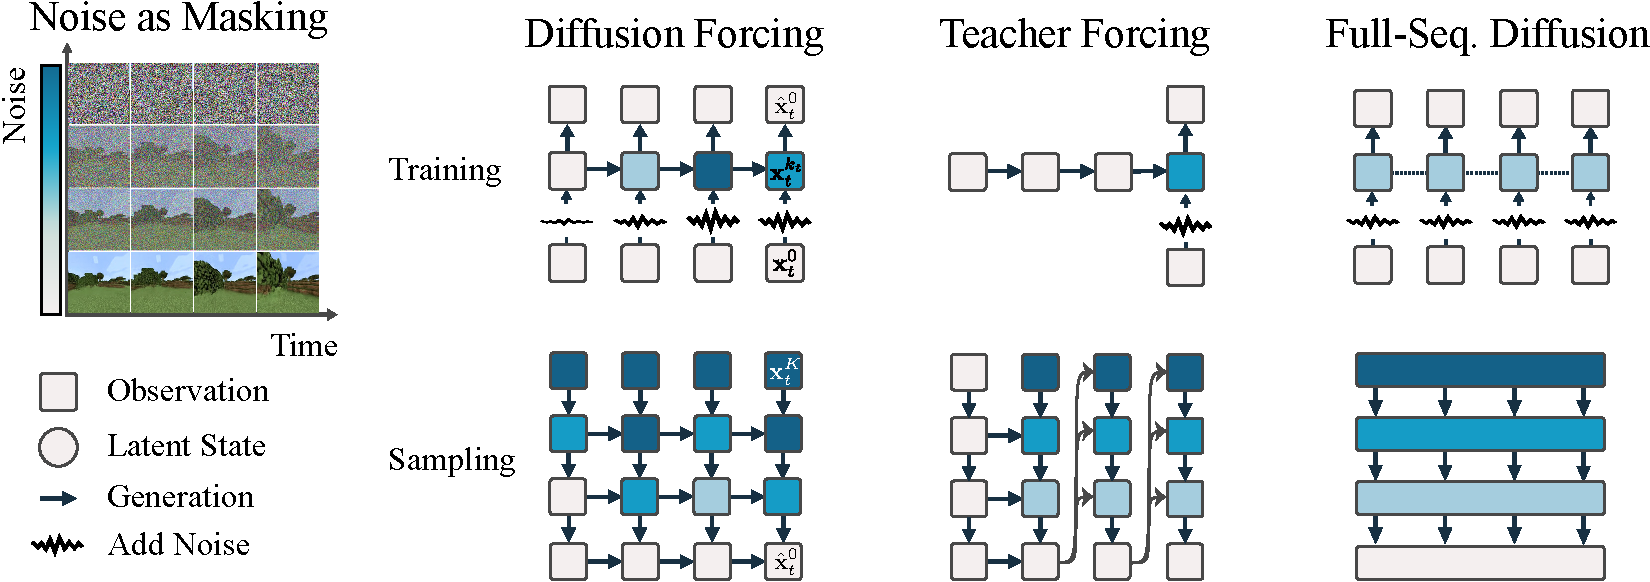
\includegraphics[width=\linewidth]{figures/pdf/Overview_best_guess.pdf}
    \caption{\textbf{Method Overview.} 
    Diffusion Forcing trains causal sequence neural networks (such as an RNN or a masked transformer) to denoise flexible-length sequences where each frame of the sequence can have a \emph{different} noise level.
    In contrast, next-token prediction models, common in language modeling, are trained to predict a single next token from a \emph{ground-truth} sequence (teacher forcing~\cite{teacher_forcing}), and full-sequence diffusion, common in video generation, train non-causal architectures to denoise all frames in a sequence at once with the \emph{same} noise level.
    \algo{} thus \emph{interleaves} the time axis of the sequence and the noise axis of diffusion, unifying strengths of both alternatives and enabling completely new capabilities (see Secs.~\ref{sec:zigzag_example},\ref{sec:method_decision_making}).
    }
    \label{fig:method}
    \vspace{-5pt}
\end{figure*}

\begin{figure}[ht]
\begin{center}
\includegraphics[width=\linewidth]{images/CogVideoX-framepacking-2.jpg}
\end{center}
\caption{
The diagram of mixed-duration training and Frame Pack. To fully utilize the data and enhance the model's generalization capability, we train on videos of different duration within the same batch.}
\label{fig:framepack}
\vspace{-5mm}
\end{figure}

\section{Training \model}

%\subsection{Setting}
We mix images and videos during training, treating each image as a single-frame video. 
Additionally, we employ progressive training from the resolution perspective. 
For the diffusion setting, we adopt v-prediction~\citep{salimans2022progressive} and zero SNR~\citep{lin2024common}, following the noise schedule used in LDM~\citep{rombach2022high}.

\subsection{Multi-Resolution Frame Pack}
Previous video training methods often involve joint training of images and videos with a fixed number of frames~\citep{singer2022make, blattmann2023stable}. 
However, this approach usually leads to two issues: 
First, there is a significant gap between the two input types using bidirectional attention, with images having one frame while videos having dozens of frames. 
We observe that models trained this way tend to diverge into two generative modes based on the token count and not to have good generalizations. %e well. 
Second, to train with a fixed duration, we have to discard short videos and truncate long videos, which prevents full utilization of the videos of varying number of frames.

To address these issues, we choose mixed-duration training, which means training videos of different lengths together. 
However, inconsistent data shapes within the batch make training difficult. 
Inspired by Patch'n Pack \citep{dehghani2024patch}, we place videos of different duration (also in different resolutions) into the same batch to ensure consistent shapes within each batch, a method we refer to as \textit{Multi-Resolution Frame Pack}. The process is illustrated in Figure~\ref{fig:framepack}. 

We use 3D RoPE to model the position relationship of various video shape. There are two ways to adapt RoPE to different resolutions and durations. One approach is to expand the position encoding table and, for each video, select the front portion of the table according to the resolution (extrapolation). The other is to scale a fixed-length position encoding table to match the resolution of the video (interpolation). Considering that RoPE is a relative position encoding, we chose the first approach to keep the clarity of model details.


\subsection{Progressive Training}
Videos from the Internet usually include a significant amount of low-resolution ones. And directly training on high-resolution videos is extremely expensive. To fully utilize data and save costs, the model is first trained on 256px videos to learn semantic and low-frequency knowledge. Then it is trained on gradually increased resolutions, from 256px to 512px, 768px, to learn high-frequency knowledge. To maintain the ability of generating videos with different aspect ratios, we keep the aspect ratio unchanged and resize the short side to above resolutions. Finally, we select a subset of high-quality videos to fine-tune the model, since the filtered pre-training data still contains a certain proportion of dirty data, such as subtitles, watermarks, and low-bitrate videos. We find this step can effectively remove generated subtitles and watermarks and improve the visual quality.
Moreover, we trained an image-to-video model based on above model. See Appendix~\ref{app:i2v} for details.
 
% (\tjy:)The training pipeline of \model is divided into three stages: low-resolution training, high-resolution training, and high-quality video fine-tuning. 
% Similar to images, videos from the Internet usually include a significant amount of low-resolution ones. 
% Progressive training can effectively utilize videos of various resolutions. 
% Moreover, training at low resolution initially can equip the model with coarse-grained modeling capabilities, followed by high-resolution training to enhance its ability to capture fine details. 
% Compared to direct high-resolution training, staged training can also help reduce the overall training time.

% \begin{figure}[h]
% \begin{center}
% \includegraphics[width=0.9\linewidth]{images/ive.jpg}
% \end{center}
% \caption{The comparison between the initial generation states of extrapolation and interpolation when increasing the resolution with RoPE encoding. Extrapolation tends to generate multiple small, clear, and repetitive images, while interpolation generates a blurry large image.}
% \label{fig:ive}
% \end{figure}

% \paragraph{Extrapolation of Position Code.}
% When adapting low-resolution position encoding to high-resolution, we consider two different methods: interpolation and extrapolation. We show the effects of two methods in Figure~\ref{fig:ive}. Interpolation tends to preserve global information more effectively, whereas the extrapolation better retains local details. Given that RoPE is a relative position encoding, We chose the extrapolation to maintain the relative position between pixels. 

% \paragraph{High-Quality Fine-Tuning.}
% Since the filtered pre-training data still contains a certain proportion of dirty data, such as subtitles, watermarks, and low-bitrate videos, we selected a subset of higher quality video data, accounting for 20\% of the total dataset, for fine-tuning in the final stage. This step effectively removed generated subtitles and watermarks and slightly improved the visual quality. However, we also observed a slight degradation in the model's semantic ability.


\subsection{Explicit Uniform Sampling}

~\citet{ho2020denoising} defines the training objective of diffusion as 
\begin{equation}~\label{eq:ddpm-loss}
    L_\mathrm{simple}(\theta) := \mathbf{E}_{t, x_0, \epsilon}{ \left\| \epsilon - \epsilon_\theta(\sqrt{\bar\alpha_t} x_0 + \sqrt{1-\bar\alpha_t}\epsilon, t) \right\|^2},
\end{equation}
where $t$ is uniformly distributed between 1 and T. 
The common practice is for each rank in the data parallel group to uniformly sample a value between 1 and $T$, which is in theory equivalent to Equation~\ref{eq:ddpm-loss}. 
However, in practice, the results obtained from such random sampling are often not sufficiently uniform, and since the magnitude of the diffusion loss is related to the timesteps, this can lead to significant fluctuations in the loss. 
Thus, we propose to use \textit{Explicit Uniform Sampling} to divide the range from 1 to $T$ into $n$ intervals, where $n$ is the number of ranks. 
Each rank then uniformly samples within its respective interval. 
This method ensures a more uniform distribution of timesteps. 
As shown in Figure~\ref{fig:subfigures} (d), the loss curve from training with Explicit Uniform Sampling is noticeably more stable. 

In addition, we compare the loss at each diffusion timestep alone between two choices for a more precise comparison. We find after using explicit uniform sampling, the loss at all timesteps decreased faster, indicating that this method can also accelerate loss convergence.
\input{posttraining.tex}
\section{Results}
\label{section:results}

We performed an extensive series of evaluations of Llama 3, investigating the performance of: \textbf{(1)} the pre-trained language model, \textbf{(2)} the post-trained language model, and \textbf{(3)} the safety characteristics of Llama 3. We present the results of these evaluations in separate subsections below. 

\input{results/pretrained.tex}
\input{results/finetuned.tex}
LLMs can propagate harmful content, reinforce biases, or amplify misinformation. While users are responsible for assessing the potential risks of generated content, developers must prioritize legal and safety considerations, strengthening models against attacks that may bypass safety protocols. 

In line with the Biden-Harris US Executive Order on AI \citep{whitehouse2023fact}, we curated the Biden-Harris Redteam Dataset, consisting of 5000 instruction-response pairs, addressing key concerns such as harm, cyber-attacks, CNBR risks, illegal acts, and privacy infringement. This dataset was created using a combination of filtering human preference data on harmlessness and template-based methods, with responses reviewed and edited for quality and safety. We used this dataset to instruction-tune \system\ and evaluated its safety levels before and after tuning. Details are provided in Section \ref{sec:experiments}, with further dataset insights in Appendix \ref{ap:safety}.

\input{inference.tex}
\input{vision.tex}
\begin{table}[h]
    % \captionsetup{font=small}
    \small
    \centering
    % \vspace{-1em}
    \caption{\label{table:speech} SC 10-class classification on raw audio (sequence length 16000).}
    %   \vspace{1em}
    {
        \begin{tabular}{@{}|cccccc|@{}}
            \hline
        %   \specialrule{.15em}{.05em}{.05em}
        H3 & S4 & WaveGan-D & Transformer & Performer & CKConv  \\ % & Training time \\
        %   \specialrule{.15em}{.05em}{.05em}
        \hline
        97.04 & \textbf{97.50} & 96.25 & x & 30.77 & 71.66 \\ \hline
        \end{tabular}
    }
    % \vspace{-1.5em}
\end{table}
\section{Related Work}
\label{sec:related_work}

\paragraph{Attention variants and distributed attention}
Ever since attention became popular with the Transformer
architecture~\citep{vaswani2017attention}, there has been a large body of work
on approximating attention to scale it to longer sequences.
These approximation methods can generally be categorized into two classes:
sparse and low-rank.
Sparse attention only computes some entries of the attention matrix ($\mathrm{softmax}(\vQ
\vK^T)$) and assumes that other entries are zero.
Different methods have different ways of choosing which entries should be zero,
either with a fixed pattern~\citep{child2019generating}, with a sliding
window~\citep{beltagy2020longformer}, or with a dynamic pattern through
hashing~\citep{kitaev2020reformer} or routing~\citep{roy2020efficient}.
The low-rank approach instead assumes that the attention matrix has a low-rank
structure, and apply a pointwise nonlinearity to the query and
key~\citep{katharopoulos2020transformers} with random
projection~\citep{choromanski2021rethinking, peng2021random, xiong2021nystromformer}.
One can also combine the sparse and low-rank approximation for better
quality~\citep{zaheer2020bigbird,scatterbrain}.
However, these approximation methods typically do not offer the same model
quality as standard attention~\citep{tay2020efficient}, and so most large-scale
models do not employ these techniques.

There are other variants of attention aimed at reducing the size of the KV cache
to improve inference efficiency. Multi-query attention~\citep{shazeer2019fast} and grouped query
attention~\citep{ainslie2023gqa} tie different heads of $\vK$ and $\vV$, and
multiple query heads interact with the same key and value head.
Multi-head latent attention~\citep{deepseekv2} parameterizes the $\vK$ and $\vV$
as low-rank projections of a shared matrix to further reduce the KV cache size.
However, all of these approaches do not change the core computation
$\mathrm{softmax}(\vQ \vK^T) \vV$ during training and simply change how $\vQ, \vK, \vV$ are
obtained.
As a result, any efficiency or accuracy improvement to the standard attention
computation benefits these methods.

To extend to even longer context, attention computation can be distributed
across multiple GPUs.
Methods such as Ring attention~\citep{liu2023ring,liu2024world} and
variants~\citep{brandon2023striped} can reach a context length of up to 1
million.
They use \fa (or \faa) as a primitive, and so the improvement from \fat would
benefit these distributed attention methods as well.

\paragraph{Alternative architectures}
Motivated by the limitations of attention, a variety of alternative
architectures have been proposed.
They build on the connection between linear
attention~\citep{katharopoulos2020transformers} and recurrent neural networks
(RNNs).
RWKV~\citep{peng2023rwkv}, H3~\citep{dao2023hungry}, MEGA~\citep{ma2023mega},
Retnet~\citep{sun2023retentive}  enhance the expressivity of the simple
cumulative sum in linear attention with more sophisticated recurrences.
Mamba~\citep{gu2023mamba} and xLSTM~\citep{beck2024xlstm} use learnable
weighting for the recurrence and can match the quality of Transformers in
language modeling at small or medium scale.
These approaches can be connected to generalizations of linear attention through
the lens of the structure of the token-mixing matrix~\citep{dao2024transformers}.
These models have started to see some traction, seeing usage in some medium to
large-scale models such as Jamba~\citep{jamba}, Zamba~\citep{zamba},
Megalodon~\citep{ma2024megalodon}, and Mamba2-hybrid~\citep{waleffe2024empirical}.
For the highest quality, these SSM- and RNN-based models still employ
many layers of attention.
We expect that techniques to speed up attention presented in this work will be
useful to speedup these alternative architectures.

\paragraph{Low-precision attention}
Quantization is a promising approach to speed up attention, but they have mostly
focused on reducing the space for KV cache for inference efficiency.
QuIP~\citep{chee2024quip} and QuIP\#\citep{tseng2024quip} use incoherent processing to reduce the quantization,
and we adapted this technique for FP8 \fat.
Recent work suggests that for inference the KV cache is highly compressible down to 4-, 3-, or
even 2-bits~\citep{hooper2024kvquant, liu2024kivi}.
However, quantization during training is still challenging as higher precision
is typically required for stable training.

\paragraph{Hardware-aware Algorithms}
Our work presented in this paper focuses on the micro-architecture
specific tuning to leverage new instruction sets and adopt a natively
asynchronous programming model. There are other orthogonal axes for
hardware-aware algorithm co-design being explored.
A recent example of this is LeanAttention~\citep{sanovar2024-leanattention},
which recognizes the poor GPU occupancy and high memory bandwidth requirements
of the sequential token generation phase as primary bottlenecks for inference
and optimizes it via a smarter load balancing strategy similar to Stream-K
load balancing~\citep{streamk} to achieve nearly peak occupancy.
There is a large literature on optimizing GEMM for specific hardware that employs
many of the same techniques.
As an example, \citet{abdel2016batched} presents a high performance batched GEMM kernel on
K40c Graphics Processing Units (GPU) for both fixed and variable sizes,
proposing specialized GEMM designs
and a comprehensive autotuning process to deliver state-of-the-art 
performance.



Hyperbolic embeddings embed hierarchical information with high
fidelity and few dimensions. We explored the limits of this approach
by describing scalable, high quality algorithms. We hope the
techniques here encourage more follow-on work on the exciting
techniques of \citet{fb, ucl}. As future work, we hope to explore how
hyperbolic embeddings can be most effectively incorporated into downstream
tasks and applications.


\clearpage
\newpage
\section*{Project Contributors}

\begin{itemize}
    % \item \textbf{Project Leaders:} AA, BB, CC
    % \item \textbf{Core Contributors:}
    % \begin{itemize}
    %     \item \textbf{Infrastructure:} AA, BB, CC
    %     \item \textbf{Data \& Recaptioning:} AA, BB, CC
    %     \item \textbf{VAE \& Model Acceleration:} AA, BB, CC
    %     \item \textbf{Model Architecture \& Algorithm \& Pre-training:} AA, BB, CC
    %     \item \textbf{Downstream Tasks:} AA, BB, CC
    % \end{itemize}
    % \item \textbf{Contributors:} AA, BB, CC, AA, BB, CC


  \item \textbf{Project Sponsors:} Jie Jiang, Yuhong Liu, Di Wang, Yong Yang 
    \item \textbf{Project Leaders:} Caesar Zhong, Hongfa Wang, Dax Zhou, Songtao Liu, Qinglin Lu, Yangyu Tao
    \item \textbf{Core Contributors:}
    \begin{itemize}
        \item \textbf{Infrastructure:} Rox Min, Jinbao Xue, Yuanbo Peng, Fang Yang, Shuai Li, Weiyan Wang, Kai Wang
        \item \textbf{Data \& Recaptioning:} Zuozhuo Dai, Xin Li, Jin Zhou, Junkun Yuan, Hao Tan, Xinchi Deng, Zhiyu He, Duojun Huang, Andong Wang, Mengyang Liu, Pengyu Li
        \item \textbf{VAE \& Model Distillation:} Bo Wu, Rox Min, Changlin Li, Jiawang Bai, Yang Li, Jianbing Wu 
        \item \textbf{Algorithm \& Model Architecture \& Pre-training:} Weijie Kong, Qi Tian, Jianwei Zhang, Zijian Zhang, Kathrina Wu, Jiangfeng Xiong, Yanxin Long
        \item \textbf{Downstream Tasks:} Jacob Song, Jin Zhou, Yutao Cui, Aladdin Wang, Wenqing Yu, Zhiyong Xu, Zixiang Zhou, Zhentao Yu, Yi Chen, Hongmei Wang, Zunnan Xu, Joey Wang, Qin Lin
    \end{itemize}
    \item \textbf{Contributors:} Jihong Zhang, Meng Chen, Jianchen Zhu, Winston Hu, Yongming Rao, Kai Liu, Lifei Xu, Sihuan Lin, Yifu Sun, Shirui Huang, Lin Niu, Shisheng Huang, Yongjun Deng, Kaibo Cao, Xuan Yang, Hao Zhang, Jiaxin Lin, Chao Zhang,  Fei You, Yuanbin Chen, Yuhui Hu, Liang Dong Zheng Fang, Dian Jiao, Zhijiang Xu
\end{itemize}



\clearpage
\newpage
\bibliographystyle{assets/plainnat}
\bibliography{paper,anthology}



\end{document}
